\documentclass[../Interim_Report_Master]{subfiles}
\begin{document}
\hypertarget{sol_meth}{\section{Single Particle Solution Method}\label{sol_meth}}
The ODEs for mass and heat transfer are coupled and non-linear making them challenging to solve analytically. To get the simulation running initially the ODEs for heat and mass transfer were solved separately. Different numerical methods were used to solve the ODEs to evaluate their suitability. 

For the purpose of this testing the model was implemented in Python. The model is contained within a single class that contains methods for evaluating the model. This is iterated through a timestepping procedure to solve the model. The code can be found at \cite{andrew_py}.

\subsection{Simulation Settings}\label{sec:sim_set}
For the uncoupled heat and mass transfer the following settings were used. 

The Reynolds number was fixed at zero, which means the drop is stationary and there is only diffusive heat transfer. This fixes the value of the Nusselt and Sherwood numbers as 2. As M1 is used $f_2=1$ and $H_{\Delta T}=0$. 

In addition to this to decouple the temperature ODE from the mass ODE, the term $\left(\frac{L_V}{C_L}\right)\frac{\dot{m_d}}{m_d}$ was ignored. The mass transfer ODE requires no such alterations to decouple it. 

Some parameters must be calculated based on empirical relations. For the droplet this includes $L_V$ and for the gas this includes $\mu_G$, $Pr_G$ and $Sc_G$. $P_G$ is determined using the ideal gas law. See Section \ref{sec:phys_data} for the relations. 

The full settings are listed in Table \ref{tab:sim_set_uc}. The conditions used are from \cite{ranz1952}.
\begin{table}[H]
	\centering
	\begin{tabular}{|l c|}
		\hline
		\textbf{Parameter} & \textbf{Setting} \\ \hline
		\textbf{Droplet Physical Properties} &  \\ 
		Molecular Weight of Vapour Phase $W_V$ & $18.015~kg/kg~mol$ \\ 
		Boiling Temperature $T_B$ & $373.15~K$ \\ 
		Density of Liquid Phase $\rho_L$ & $997~kg/m^3$ \\
		Specific Heat Capacity of Liquid Phase $C_L$ & $4184~J/(kg~K)$ \\ 
		Initial Temperature $T_{d0}$ & $282~K$ \\ 
		Initial Diameter $D_0$ & $\sqrt{1.1}~mm$ \\ 
		Initial Reynolds Number $Re_0$ & $0$ \\ \hline
		\textbf{Gas Properties} &  \\ 
		Molecular Weight of Phase $W_C$ & $28.97~kg/(kg~mol)$ \\ 
		Temperature $T_G$ & $298~K$ \\
		Density $\rho_G$ & $1.184~kg~m^{-3}$ \\ 
		Specific Heat for Constant Pressure $C_{P,G}$ & $1007~J~kg~K$ \\
		Free Stream Vapour Mass Fraction $Y_G$ & $0$ \\ \hline
		\textbf{Atmospheric Properties} &  \\ 
		Pressure $P_{atm}$ & $101325~Pa$ \\ \hline
		\textbf{Physical Constants} &  \\ 
		Gas Constant $\bar{R}$ & $8314.5~J/(K(kg~mol))$ \\ 
		Universal Gas Constant $R$ & $287~J/(kg~K)$ \\ \hline
		\textbf{Simulation Properties} &  \\ 
		Correction factor $f_2$ & 1 \\
		Driving Potential $H_{\Delta T}$ & 0 \\ \hline
	\end{tabular}
	\caption{Simulation settings used for evaluating the numerical methods.}
	\label{tab:sim_set_uc}
\end{table}

The timestep size used is included in the results.

\subsection{Uncoupled Heat Transfer}
\subsubsection{Analytic Solution}
Using the settings specified in Section \ref{sec:sim_set} the temperature ODE becomes:
\begin{equation}
\frac{dT_{d}}{dt} = \frac{f_{2}Nu}{3Pr_{G}}\left(\frac{\theta_1}{\tau_d}\right)(T_{G}-T_{d})
\label{temp_transfer_simple}
\end{equation}

Which can be solved analytically to provide a reference point for the numerical solution. See Section \ref{uc_heat_dev} for the full derivation which produces the solution:
\begin{equation}
T_{d_{n+1}} = T_G - (T_G-T_{d_{n}})e^{-\left(\frac{f_{2}Nu}{3Pr_{G}}\left(\frac{\theta_1}{\tau_d}\right)\right)\Delta t}
\label{heat_sol_an}
\end{equation}

\subsubsection{Results}
The implementation of equation \ref{temp_transfer_simple} requires the usage of a for loop to iterate through the time steps. Importantly, this loop must check to see if $T_{d_{n}}$ has exceeded $T_G$, if this condition is met the loop must stop as the following results will be unphysical. 

For plotting data the results have been non-dimensionalised. The points in time are non-dimensionalised with the particle heat transfer time constant $\tau_h$. the temperature values can be non-dimensionalised with the steady state temperature by solving the uncoupled heat transfer equation for $T_d$ when $dT/dt$ is zero:
\begin{subequations}
\begin{align}
\frac{dT_{d}}{dt} &= \frac{f_{2}Nu}{3Pr_{G}}\left(\frac{\theta_1}{\tau_d}\right)(T_{G}-T_{d}) \\
0 &= \frac{f_{2}Nu}{3Pr_{G}}\left(\frac{\theta_1}{\tau_d}\right)(T_{G}-T_{d}) \\
T_d &= T_G
\end{align}
\end{subequations}

The results from a simulation run for one droplet of water evaporating in air for a time step of $\tau_d$ are shown in Figure \ref{temp_time_tau}. 
\begin{figure}[H]
	\centering
	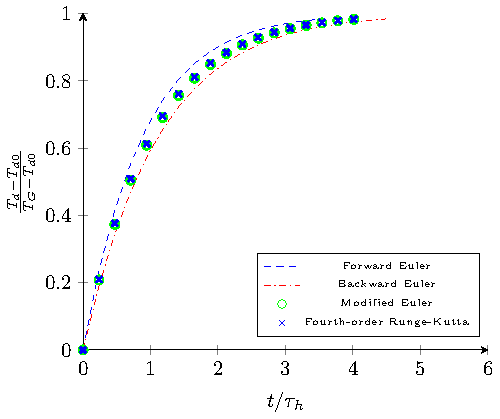
\includegraphics[width=0.8\textwidth]{./Diagrams/Uncoupled_Heat_Transfer_tau/Uncoupled_Heat_Transfer_tau.pdf}
	\caption{$T_d$ for a droplet sized $D^2=1.1mm$ with $Re_d=0$, $T_{d_0}=282K$, $T_G=298K$ and $\Delta t=\tau_d$.}
	\label{temp_time_tau}
\end{figure}

As expected the first order implicit and explicit methods undershoot and overshoot the analytic solution respectively. This is because an explicit method makes an estimate of what the next value will be based on the current gradient. Given the gradient of the analytic solution is always decreasing this means the explicit method is always overestimating the value at the next timestep. A similar argument can be made for an implicit method.

It can also be seen from Figure \ref{temp_time_tau} the droplet heats up to the gas temperature within just over $4\tau_h$. As $1/e^4$ is $\approx 2\%$ and the simulation stops once the droplet temperature has reached $99.9\%$ of the gas temperature this proves the droplet temperature increases at the correct rate.

The timestep for example be halved to $\tau/2$ as in Figure \ref{temp_time_tau_2}.
\begin{figure}[H]
	\centering
	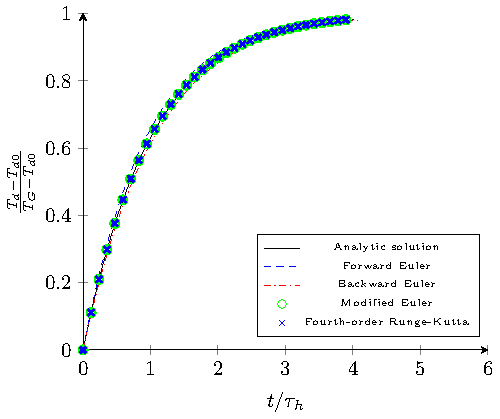
\includegraphics[width=0.8\textwidth]{./Diagrams/Uncoupled_Heat_Transfer_tau_2/Uncoupled_Heat_Transfer_tau_2.pdf}
	\caption{$T_d$ for a droplet sized $D^2=1.1mm$ with $Re_d=0$, $T_{d_0}=282K$, $T_G=298K$ and $\Delta t=\tau/2$.}
	\label{temp_time_tau_2}
\end{figure}

Figure \ref{temp_time_tau_2} shows the numerical solutions are closer to the analytic solution compared with Figure \ref{temp_time_tau}. Therefore demonstrating the numerical solutions converge to the analytic solution as expected. 

\newpage

\subsubsection{Comparison of Numerical Methods}
The convergence of numerical results to the analytic solution for decreasing timesteps is highlighted by Figure \ref{uc_temp_convergence}.
\begin{figure}[H]
	\centering
	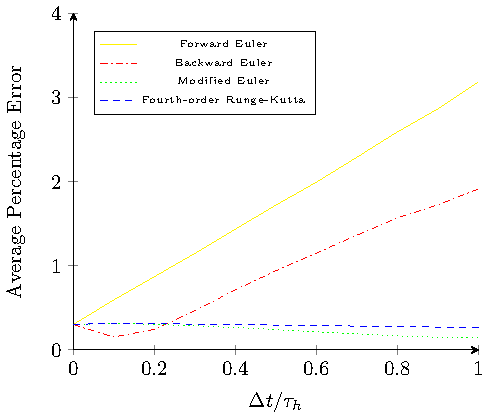
\includegraphics[width=0.8\textwidth]{./Diagrams/Uncoupled_Temp_Convergence/Uncoupled_Temp_Convergence.pdf}
	\caption{Average percentage error compared with the analytic solution for a range of timesteps and numerical methods.}
	\label{uc_temp_convergence}
\end{figure}

For a timestep very close to zero all the numerical methods appear to have the same average percentage error. This should be zero but is actually $0.3\%$. This is quite an unusual result, especially when considering the average percentage error decreases with increasing timestep for the modified Euler and Runge-Kutta methods. 

This turned out to be a bug in the method used for benchmarking the statistics. The error was that  The simulation stops once $T_d = 0.999T_G$. Removing this stop condition and fixing the simulation lengths using the max number of timesteps produces statistics that make sense:
\begin{figure}[H]
	\centering
	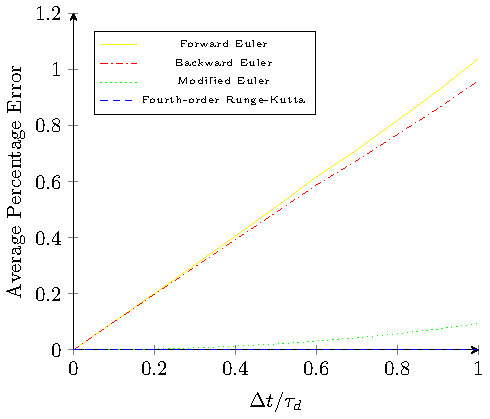
\includegraphics[width=0.8\textwidth]{./Diagrams/Uncoupled_Temp_Convergence_2/Uncoupled_Temp_Convergence_2.pdf}
	\caption{Average percentage error compared with the analytic solution for a range of timesteps and numerical methods.}
	\label{uc_temp_convergence_2}
\end{figure}

The simulation duration was fixed to $\tau_d$ and the number of timesteps calculated by dividing this by the timestep size. As Figure \ref{uc_temp_convergence_2} shows all methods converge to zero error with a timestep size of zero. The forward Euler method has perfect linearity with a $R^2$ value of $0.9998$ as calculated by Excel. The backward Euler method has a slightly smaller error, but again has good linearity with $R^2=0.9996$. The modified Euler and Runge-Kutta methods now have noticeably different gradients for their error plots. It is just possible to distinguish that the modified Euler method has a quadratic error function, with $R^2=0.9996$. Due to how small the average percentage error of the Runge-Kutta method is this has also been plotted separately on Figure \ref{uc_temp_convergence_3}.
\begin{figure}[H]
	\centering
	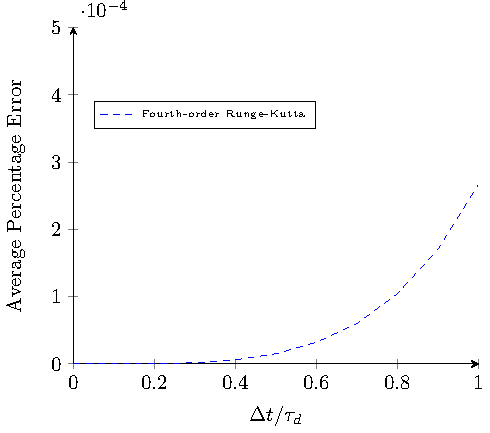
\includegraphics[width=0.8\textwidth]{./Diagrams/Uncoupled_Temp_Convergence_2/Uncoupled_Temp_Convergence_3.pdf}
	\caption{Average percentage error compared with the analytic solution for the Runge-Kutta method for a range of timesteps.}
	\label{uc_temp_convergence_3}
\end{figure}

The average percentage error as a function of the timestep for the Runge-Kutta method is a quartic as expected given the method is fourth-order. The statistics are again well behaved with $R^2=1.000$. 

$R^2$ values close to $1$ demonstrate the numerical methods have been implemented correctly as their results are to the correct order. Moreover, as the results for all numerical methods converge to the analytic solution for decreasing timestep size this verifies they are solving the uncoupled temperature case correctly.

\newpage

\subsection{Uncoupled Mass Transfer}\label{sec:uc_mass}
\subsubsection{Analytic Solution}
The mass transfer equation is:
\begin{equation}
\frac{dm_d}{dt} = -\frac{Sh}{3Sc_G}\frac{m_d}{\tau_d}H_M
\label{mass3}
\end{equation}

Unlike the uncoupled temperature equation, equation \ref{mass3} requires some rearrangement before it can be solved. The term $\tau_d$ contains diameter which is a function of mass so this must be taken into account. In addition to this, the literature commonly plots $D^2$ instead of mass; solving equation \ref{mass3} for diameter is possible and this is outlined in Section x. However, here equation \ref{mass3} will solved for $m_d$ and for plotting data the mass can be converted to $D^2$. In either solution case a relation between diameter and mass is needed.

Using the relation between mass, density and volume:
\begin{subequations}
\begin{align}
m_d = & \rho V_d \\
m_d =& \rho_d \left(\frac{4}{3}\right) \pi \left(\frac{D}{2}\right)^3 \\
m_d =& \frac{\rho_d \pi D^3}{6} \\
D = & \left(\frac{6}{\rho_d \pi}\right)^{1/3} \left(m_d\right)^{1/3}
\end{align}
\end{subequations}
 
Therefore, substituting this relation into \ref{mass3} yields:
\begin{subequations}
\begin{align}
\frac{dm_d}{dt} =& -\frac{Sh}{3Sc_G}\frac{m_d}{\tau_d}H_M \\
\frac{dm_d}{dt} =& -\frac{Sh}{3Sc_G} H_M m_d\left(\frac{18\mu_G}{\rho_d D^2}\right)\\
\frac{dm_d}{dt} =& -\frac{Sh}{3Sc_G} H_M m_d\left(\frac{18\mu_G}{\rho_d}\right)\left(\left(\frac{6}{\rho_d \pi}\right)^{-2/3} \left(m_d\right)^{-2/3}\right) \\ 
\frac{dm_d}{dt} =& -\frac{Sh}{Sc_G}\mu_G H_M \left(\frac{6}{\rho_d}\right)^{1/3}\pi^{2/3} m_d^{1/3}
\end{align}
\end{subequations}

The full solution as outlined in Section \ref{sec:mass_sol} gives:
\begin{equation}
\left({m_d}_{n+1}\right)^{2/3} = \left({m_d}_{n}\right)^{2/3} - \frac{2Sh}{3Sc_G}\mu_G H_M \left(\frac{6}{\rho_d}\right)^{1/3}\pi^{2/3} ~ \Delta t
\end{equation}

\subsubsection{Results}
The mass transfer results have been plotted in Figure \ref{diameter_squared_time_tau} for $\Delta t=\tau_d$. For the numerical solution $\tau_d$ was recalculated at the start of each timestep. At the end of each timestep the mass value is used to calculate $D^2$, which is non-dimensionalised with the initial diameter. The results from the modified Euler and Runge-Kutta methods have been plotted separately on Figure \ref{diameter_squared_time_2_tau}.
\begin{figure}[H]
	\centering
	\begin{subfigure}{\textwidth}
		\centering
		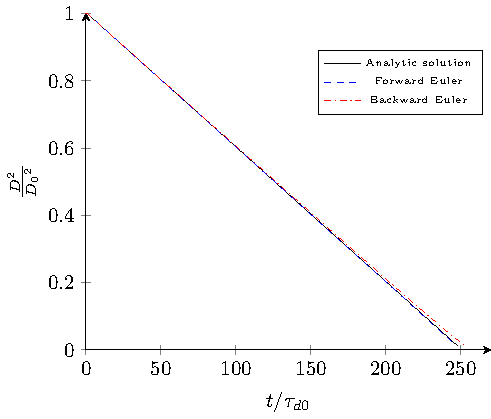
\includegraphics[width=0.8\textwidth]{./Diagrams/Uncoupled_D2_Transfer_tau/Uncoupled_D2_Transfer_tau.pdf}
		\caption{}
		\label{diameter_squared_time_tau}
	\end{subfigure}
\end{figure}
\begin{figure}\ContinuedFloat
	\centering
	\begin{subfigure}{\textwidth}
		\centering
		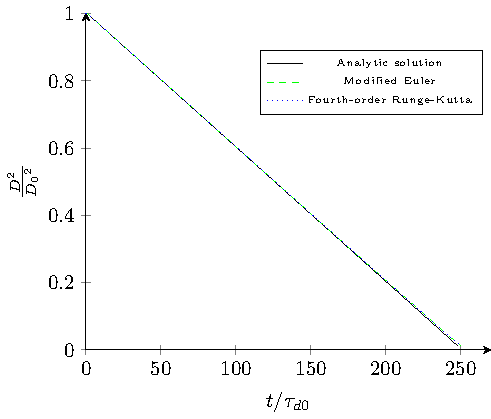
\includegraphics[width=0.8\textwidth]{./Diagrams/Uncoupled_D2_Transfer_tau/Uncoupled_D2_Transfer_2_tau.pdf}
		\caption{}
		\label{diameter_squared_time_2_tau}
	\end{subfigure}
	\caption{Non-dimensionalised $D^2$ for a droplet sized $D_0=\sqrt{1.1}mm$ with $Re_d=0$, $T_{d_0}=282K$, $T_G=298K$ and $\Delta t=\tau_d$.}
\end{figure}

Much like was the case for the temperature solution the explicit methods overshoot the analytic solution. The exception being the forward Euler method under-predicts the analytic solution and appears to better predict the the analytic solution. The droplet evaporation time has been non-dimensionalised with the initial droplet momentum timescale as this changes as the droplet's mass decreases.

Note that unlike the heat transfer solution the results of the mass transfer plotted as diameter squared give a linear relation. This is intrinsic to the assumption the droplet temperature remains at the wet bulb temperature. Therefore the rate of evaporation is only dependent on surface area which is a function of $D^2$.

\subsubsection{Comparison of Numerical Methods}
To confirm the numerical methods converge to the analytic solution a similar convergence plot to Figure \ref{uc_temp_convergence_2} has been plotted in Figure \ref{uc_d2_convergence}. For this convergence test the simulation time was limited by the mass stop condition.
\begin{figure}[H]
	\centering
	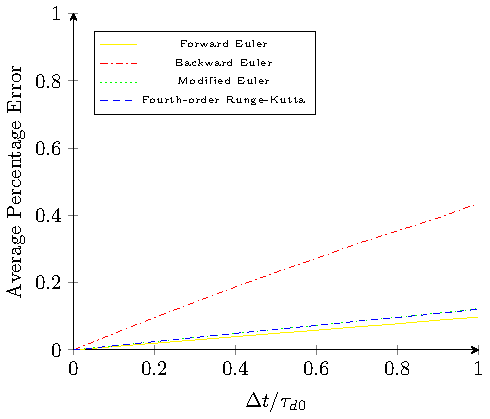
\includegraphics[width=0.8\textwidth]{./Diagrams/Uncoupled_D2_Convergence/Uncoupled_D2_Convergence.pdf}
	\caption{Average percentage error compared with the analytic solution for a range of numerical methods and timesteps.}
	\label{uc_d2_convergence}
\end{figure}

As should be the case all the numerical methods converge to zero percentage error for a timestep of zero. What is unusual is the modified Euler and Runge-Kutta methods have a slightly larger error than the forward Euler method. This may be because the high order methods are multistep. At each step within the method a prediction about what the solution is, is made. For all steps the same $\tau_d$ is used. This would explain why the modified Euler and Runge-Kutta methods have such similar error functions.

This can be fixed by updating $\tau_d$ for each step which as can be seen in Figure \ref{uc_d2_convergence_2} and \ref{uc_d2_convergence_3} the error functions are now as expected.

\begin{figure}[H]
	\centering
	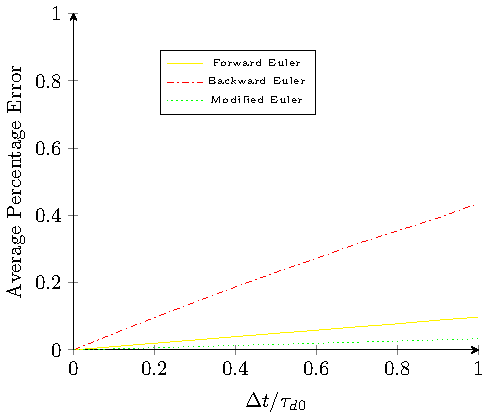
\includegraphics[width=0.8\textwidth]{./Diagrams/Uncoupled_D2_Convergence_2/Uncoupled_D2_Convergence_2.pdf}
	\caption{Average percentage error compared with the analytic solution for a range of numerical methods and timesteps.}
	\label{uc_d2_convergence_2}
\end{figure}

\begin{figure}[H]
	\centering
	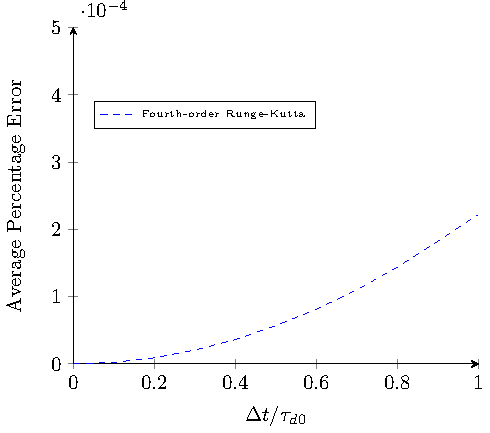
\includegraphics[width=0.8\textwidth]{./Diagrams/Uncoupled_D2_Convergence_2/Uncoupled_D2_Convergence_3.pdf}
	\caption{Average percentage error compared with the analytic solution for the Runge-Kutta method and a range of timesteps.}
	\label{uc_d2_convergence_3}
\end{figure}

Like with the temperature convergence the $R^2$ values for the $D^2$ error functions can be calculated. They are as follows:
\begin{itemize}
	\item Forward Euler - $R^2=0.9976$
	\item Backward Euler - $R^2=0.9999$
	\item Modified Euler - $R^2=1.000$
	\item Runge-Kutta - $R^2=1.000$
\end{itemize}

This affirms the numerical methods perform as expected.

The verification tests here confirm the importance of verifying simulation code to find bugs.

\subsection{Coupled Heat and Mass Transfer}
Solving the heat and mass transfer ODEs coupled is not a trivial task due to their non-linear nature. An analytic solution for the heat and mass transfer ODEs coupled has not been found so the equations can only be solved numerically. 

The simulation settings used are as per Table \ref{tab:sim_set_uc}. 

\subsubsection{Results}
The testing procedure is the same as for the uncoupled cases. With multiple numerical methods and timestep sizes being tested.

Figures \ref{coupled_d2_tau_8} and \ref{coupled_heat_tau_8} show the results for the mass and heat transfer.
\begin{figure}[H]
	\centering
	\begin{subfigure}{\textwidth}
		\centering
		\includegraphics[width=0.8\textwidth]{./Diagrams/Coupled_Heat_Mass_Transfer_tau_8/Coupled_d2_Transfer_tau_8.pdf}
		\caption{}
		\label{coupled_d2_tau_8}
	\end{subfigure}
\end{figure}
\begin{figure}\ContinuedFloat
	\centering
	\begin{subfigure}{\textwidth}
		\centering
		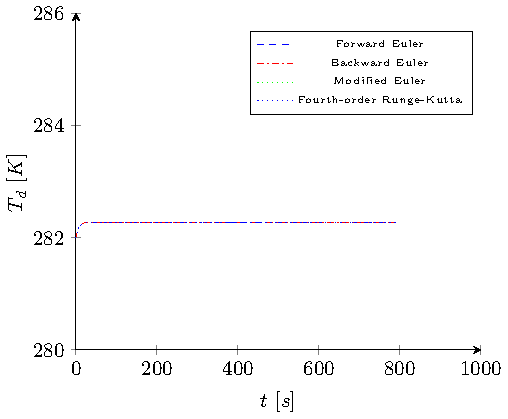
\includegraphics[width=0.8\textwidth]{./Diagrams/Coupled_Heat_Mass_Transfer_tau_8/Coupled_Heat_Transfer_tau_8.pdf}
		\caption{}
		\label{coupled_heat_tau_8}
	\end{subfigure}
	\caption{Droplet diameter squared (a) and droplet temperature (b) temporal evolution for a water droplet sized $D_0=\sqrt{1.1}mm$ with $Re_d=0$, $T_{d_0}=282K$, $T_G=298K$ and $\Delta t=\tau_d/8$.}
\end{figure}

The droplet quickly reaches an equilibrium temperature of $282.27K$ and remains at this temperature as the droplet evaporates at a steady rate. There is little variation between the numerical methods.

\subsubsection{Comparison of Numerical Methods}
Increasing the size of the timestep makes the difference between the numerical methods more evident. Using a timestep of $\tau_d/2$ it can be seen the explicit methods diverge quite significantly at the end of the simulation in Figures \ref{coupled_d2_tau_2} and \ref{coupled_heat_tau_2}. 
\begin{figure}[H]
	\centering
	\begin{subfigure}{\textwidth}
		\centering
		\includegraphics[width=0.8\textwidth]{./Diagrams/Coupled_Heat_Mass_Transfer_tau_2/Coupled_d2_Transfer_tau_2.pdf}
		\caption{}
		\label{coupled_d2_tau_2}
	\end{subfigure}
\end{figure}
\begin{figure}\ContinuedFloat
	\centering
	\begin{subfigure}{\textwidth}
		\centering
		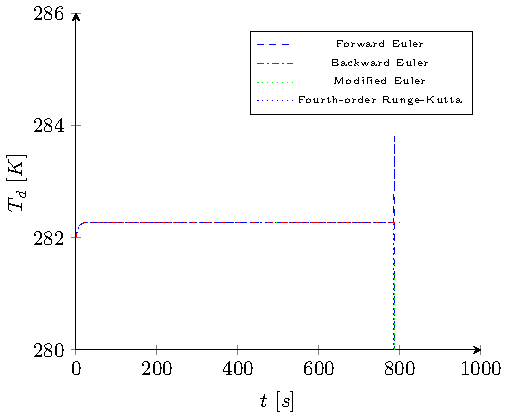
\includegraphics[width=0.8\textwidth]{./Diagrams/Coupled_Heat_Mass_Transfer_tau_2/Coupled_Heat_Transfer_tau_2.pdf}
		\caption{}
		\label{coupled_heat_tau_2}
	\end{subfigure}
	\caption{Droplet diameter squared (a) and droplet temperature (b) temporal evolution for a water droplet sized $D_0=\sqrt{1.1}mm$ with $Re_d=0$, $T_{d_0}=282K$, $T_G=298K$ and $\Delta t=\tau_d/2$.}
\end{figure}

Plotting the results non-dimensionally in Figure \ref{coupled_d2_tau_2_nd} and \ref{coupled_heat_tau_2_nd} using $\tau_d$ makes it clear what causes this:
\begin{figure}[H]
	\centering
	\begin{subfigure}{\textwidth}
		\centering
		\includegraphics[width=0.8\textwidth]{./Diagrams/Coupled_Heat_Mass_Transfer_tau_2_nd/Coupled_d2_Transfer_tau_2_nd.pdf}
		\caption{}
		\label{coupled_d2_tau_2_nd}
	\end{subfigure}
\end{figure}
\begin{figure}\ContinuedFloat
\centering
\begin{subfigure}{\textwidth}
	\centering
	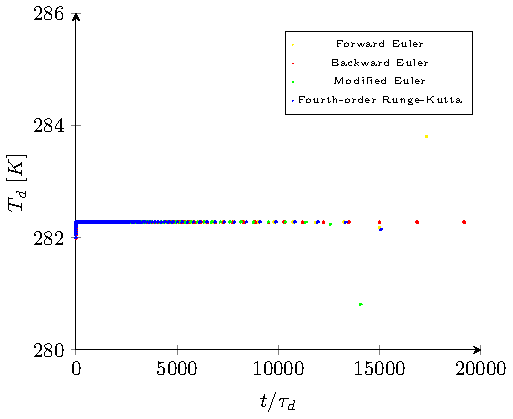
\includegraphics[width=0.8\textwidth]{./Diagrams/Coupled_Heat_Mass_Transfer_tau_2_nd/Coupled_Heat_Transfer_tau_2_nd.pdf}
	\caption{}
	\label{coupled_heat_tau_2_nd}
\end{subfigure}
\caption{Droplet diameter squared (a) and droplet temperature (b) temporal evolution for a water droplet sized $D_0=\sqrt{1.1}mm$ with $Re_d=0$, $T_{d_0}=282K$, $T_G=298K$ and $\Delta t=\tau_d/2$. The time axis is non-dimensionalised with $\tau_d$.}
\end{figure}

The momentum timescale of the droplet, $\tau_d$ decreases as the droplet diameter decreases. This means the timescale of the physics increases relative to the size of the timestep as the ODEs are a function of $1/\tau_d$. As explicit methods extrapolate based on the current value to find the next value; the error incurred in the extrapolation increases with the size of timestep. A possible solution to this problem is dynamic timestepping which involves changing the size of the timestep as a function of $\tau_d$. For one droplet this procedure is simple enough, but for multiple droplets the timestep is common across all droplets. This means basing the timestep size on the smallest droplet timescale, which could be very inefficient. Consider a scenario where one droplet at the start of the simulation a droplet rapidly evaporates, this means a small timestep size for droplets which may be very slowly evaporating. 

Therefore, the required solution is to use an implicit method. The backward Euler method is appropriate to use here given it does not suffer the same instability as the explicit methods. Further, it permits the usage of larger timesteps which is advantageous in reducing computation time. Higher order implicit methods are available, but at the cost of an iterative procedure at each timestep to solve the equations. Therefore the implicit Euler method will be used for the OpenCL simulation code. 

\subsection{Coupled Heat and Mass Transfer Validation}\label{sec:heat_mass_val}
As a suitable procedure has been chosen for running the simulation the procedure can be validated using a further two common test cases found in the literature. The first is the evaporation of a hexane droplet using the conditions from \cite{Downing1966}. These are outlined in Table \ref{tab:sim_set_hex}. 
\begin{table}[H]
	\centering
	\begin{tabular}{|l c|}
		\hline
		\textbf{Parameter} & \textbf{Setting} \\ \hline
		\textbf{Droplet Physical Properties} &  \\ 
		Molecular Weight of Vapour Phase $W_V$ & $86.178~kg/kg~mol$ \\ 
		Boiling Temperature $T_B$ & $447.7~K$ \\ 
		Density of Liquid Phase $\rho_L$ & $664~kg/m^3$ \\
		Specific Heat Capacity of Liquid Phase $C_L$ & $2302~J/(kg~K)$ \\ 
		Initial Temperature $T_{d0}$ & $281~K$ \\ 
		Initial Diameter $D_0$ & $1.76~mm$ \\ 
		Reynolds Number $Re_d$ & $110$ \\ \hline
		\textbf{Gas Properties} &  \\ 
		Molecular Weight of Phase $W_C$ & $28.97~kg/(kg~mol)$ \\ 
		Temperature $T_G$ & $437~K$ \\
		Density $\rho_G$ & $0.807~kg~m^{-3}$ \\ 
		Specific Heat for Constant Pressure $C_{P,G}$ & $1020~J~kg~K$ \\
		Free Stream Vapour Mass Fraction $Y_G$ & $0$ \\ \hline
		\textbf{Atmospheric Properties} &  \\ 
		Pressure $P_{atm}$ & $101325~Pa$ \\ \hline
		\textbf{Physical Constants} &  \\ 
		Gas Constant $\bar{R}$ & $8314.5~J/(K(kg~mol))$ \\ 
		Universal Gas Constant $R$ & $287~J/(kg~K)$ \\ \hline
		\textbf{Simulation Properties} &  \\ 
		Correction factor $f_2$ & 1 \\
		Driving Potential $H_{\Delta T}$ & 0 \\
		Timestep Size $\Delta t$ & $\tau_{d,0}/64$ \\ \hline
	\end{tabular}
	\caption{Simulation settings used for the hexane droplet simulation.}
	\label{tab:sim_set_hex}
\end{table}

\begin{figure}[H]
	\centering
	\begin{subfigure}{\textwidth}
		\centering
		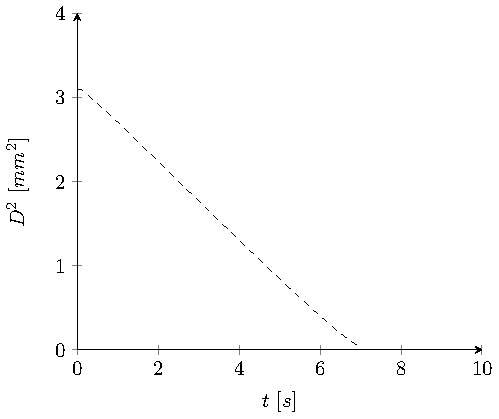
\includegraphics[width=0.8\textwidth]{./Diagrams/Coupled_Heat_Mass_Transfer_Hexane/Coupled_D2_Transfer_Hexane.pdf}
		\caption{}
		\label{coupled_d2_hexane_py}
	\end{subfigure}
\end{figure}
\begin{figure}\ContinuedFloat
	\centering
	\begin{subfigure}{\textwidth}
		\centering
		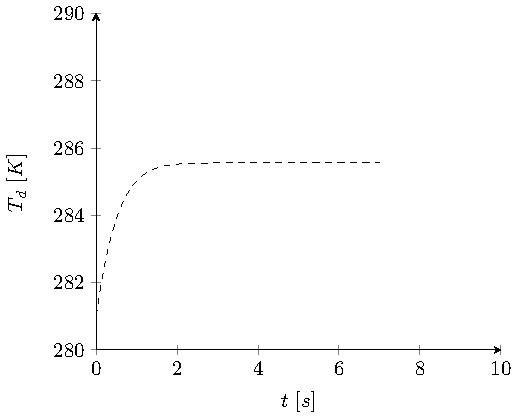
\includegraphics[width=0.8\textwidth]{./Diagrams/Coupled_Heat_Mass_Transfer_Hexane/Coupled_Heat_Transfer_Hexane.pdf}
		\caption{}
		\label{coupled_heat_hexane_py}
	\end{subfigure}
	\caption{Droplet diameter squared (a) and droplet temperature (b) temporal evolution for a hexane droplet sized $D_0=1.76mm$ with $Re_d=110$, $T_{d_0}=281$, $T_G=437$ and $\Delta t=\tau_{d0}/64$.}
\end{figure}

As with the results of M1 in the literature the model over predicts droplet evaporation rate. Nevertheless, despite the lack of usage of the ``1/3 rule'' the results are quite similar to that in \cite{Miller1998} in terms of droplet evaporation rate. However, the model appears to reach a lower equilibrium droplet temperature.

The second validation simulation is for an evaporating decane droplet and uses the conditions from \cite{wong1992}. The simulation settings are outlined in Table \ref{tab:sim_set_dec}.
\begin{table}[H]
	\centering
	\begin{tabular}{|l c|}
		\hline
		\textbf{Parameter} & \textbf{Setting} \\ \hline
		\textbf{Droplet Physical Properties} &  \\ 
		Molecular Weight of Vapour Phase $W_V$ & $142~kg/kg~mol$ \\ 
		Boiling Temperature $T_B$ & $447.7~K$ \\ 
		Density of Liquid Phase $\rho_L$ & $642~kg/m^3$ \\
		Specific Heat Capacity of Liquid Phase $C_L$ & $2520.5~J/(kg~K)$ \\ 
		Initial Temperature $T_{d0}$ & $315~K$ \\ 
		Initial Diameter $D_0$ & $2.0~mm$ \\ 
		Reynolds Number $Re_d$ & $17$ \\ \hline
		\textbf{Gas Properties} &  \\ 
		Molecular Weight of Phase $W_C$ & $28.97~kg/(kg~mol)$ \\ 
		Temperature $T_G$ & $1000~K$ \\
		Density $\rho_G$ & $0.3529~kg~m^{-3}$ \\ 
		Specific Heat for Constant Pressure $C_{P,G}$ & $1141~J~kg~K$ \\
		Free Stream Vapour Mass Fraction $Y_G$ & $0$ \\ \hline
		\textbf{Atmospheric Properties} &  \\ 
		Pressure $P_{atm}$ & $101325~Pa$ \\ \hline
		\textbf{Physical Constants} &  \\ 
		Gas Constant $\bar{R}$ & $8314.5~J/(K(kg~mol))$ \\ 
		Universal Gas Constant $R$ & $287~J/(kg~K)$ \\ \hline
		\textbf{Simulation Properties} &  \\ 
		Correction factor $f_2$ & 1 \\
		Driving Potential $H_{\Delta T}$ & 0 \\
		Timestep Size $\Delta t$ & $\tau_{d,0}/64$ \\ \hline
	\end{tabular}
	\caption{Simulation settings used for the hexane droplet simulation.}
	\label{tab:sim_set_dec}
\end{table}

The results presented in Figure \ref{coupled_d2_decane_py} and \ref{coupled_heat_decane_py} show that like for the hexane case the model performs similarly to the common implementation of M1 in the literature. Again, the model over predicts the evaporation rate compared with experimental data. Although, it fairs much better compared with the experimental data when considering the droplet temperature.
\begin{figure}[H]
	\centering
	\begin{subfigure}{\textwidth}
		\centering
		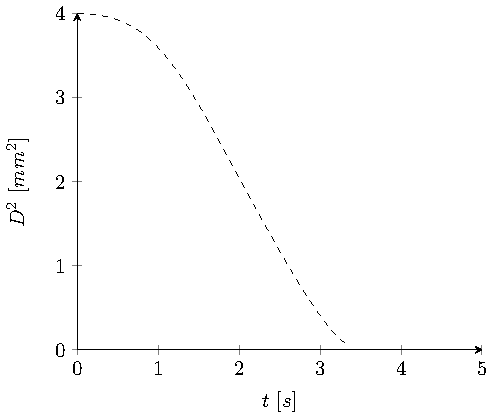
\includegraphics[width=0.8\textwidth]{./Diagrams/Coupled_Heat_Mass_Transfer_Decane/Coupled_D2_Transfer_Decane.pdf}
		\caption{}
		\label{coupled_d2_decane_py}
	\end{subfigure}
\end{figure}
\begin{figure}\ContinuedFloat
	\centering
	\begin{subfigure}{\textwidth}
		\centering
		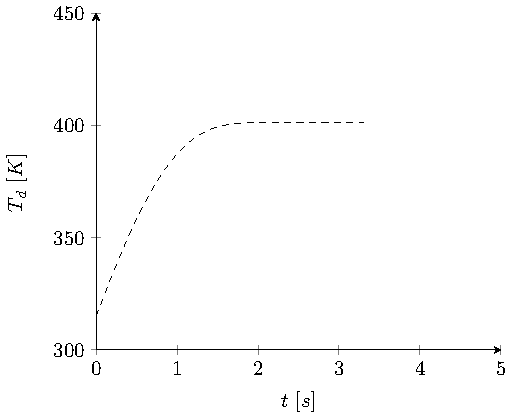
\includegraphics[width=0.8\textwidth]{./Diagrams/Coupled_Heat_Mass_Transfer_Decane/Coupled_Heat_Transfer_Decane.pdf}
		\caption{}
		\label{coupled_heat_decane_py}
	\end{subfigure}
	\caption{Droplet diameter squared (a) and droplet temperature (b) temporal evolution for a decane droplet sized $D_0=2.0mm$ with $Re_d=17$, $T_{d_0}=315K$, $T_G=1000K$ and $\Delta t=\tau_{d0}/64$.}
\end{figure}
\end{document}